%24/03 - Alberto Rastrojo
\chapter{Ensamblaje de novo}
\section{Introducción a la metagenómica}
La definición de 1998 es que la metagenómica es el estudio del material genético obtenido de muestras ambientales. En el 2005 se actualizó a la aplicación de técnicas genómicas modernas sin la necesidad de aislar y cultivar en el laboratorio las especies individuales. 

Las muestas ambientales pueden ser desde agua de mar, tierra, etc, pero también se incluyen muestras de microorganismos asociados a humanos (microbiota intestinal, vaginal, cutánea, etc.). Esto no está restringido a humanos, pudiendo extrapolarlo a plantas y otros animales. En este caso, se denomina muestra asociada a hospedador y no ambiental. 

La metagenómica permite estudiar quién está ahí, qué hacen y cómo lo hacen. Las aplicaciones principales incluyen:
\begin{itemize}
\item Biodiversidad
\item Evolución de los microorganismos
\item Ecología global (ciclos geoquímicos del carbono, producción de oxígeno, etc.)
\item Microbiota humana y otros animales (implicación en enfermedades)
\item Microbiota de las plantas (simbiosis y mejora de cultivos)
\item Bioremediación (reciclaje de aguas residuales y otros residuos)
\item Búsqueda de nuevas enzimas para la industria (biocombustibles, etc.)
\end{itemize}

Así, la definición queda de la siguiente forma: «La metagenómica es el estudio del material genético recuperado directamente de muestras ambientales mediante técnicas genómicas modernas sin necesidad de aislar y cultivar en laboratorio especies individuales». Esto antes se denominaba ecología microbiana. 

La ecología microbiana clásica se basaba en la obtención de muestras ambientales, aislamiento y purificación de microorganismos y cultivo de los mismos para su análisis. Se realizan análisis morfológicos y tinciones, análisis bioquímico, etc. El problema es que la mayoría de los microorganismos no se pueden cultivar. 

La metagenómica se impulsó gracias al descubrimiento del 16S como marcador filogenético y la PCR (polymerase chain reaction). Además, surgieron las tecnologías de secuenciación NGS. 

\begin{figure}[h]
\centering
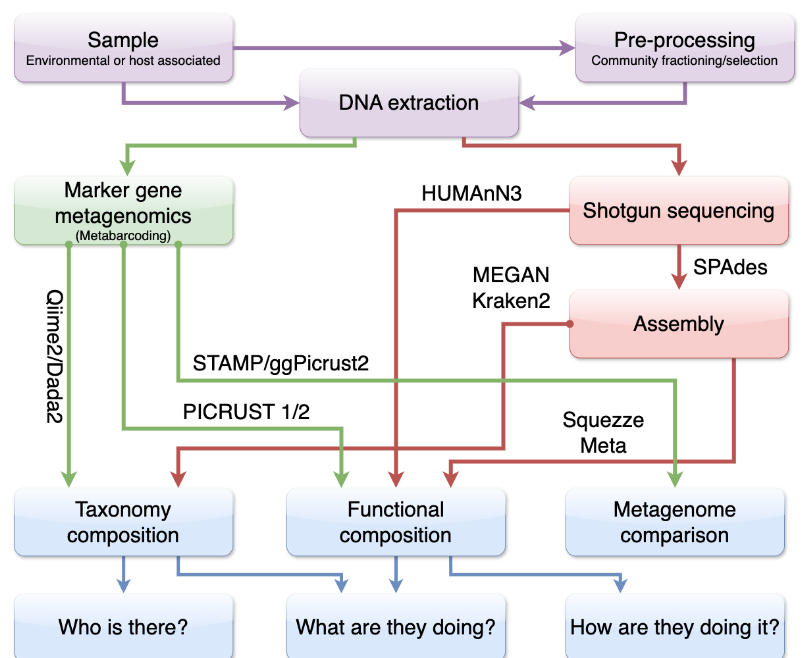
\includegraphics[width = 0.7\textwidth]{figs/metagenomics-flow.png}
\end{figure}

\section{Ensamblajes de novo}
Un contig (de contiguous) es un conjunto de segmentos de ADN superpuestos que juntos representan una región consenso de ADN.

Hay dos tipos de ensambladores:
\begin{itemize}
\item \textbf{Ensambladores basados en OLC (overlap, layout, consensus):}
\begin{itemize}
\item Celera: Ensamblador con el mejor gráfico de solapamiento (CABOG). Diseñado para secuencias Sanger, pero funciona con 454 y lecturas PacBio corregidas de errores. 
\item Newbler, también conocido como GS de novo Assembler. Diseñado para secuencias 454, pero funciona con lecturas Sanger.
\end{itemize}

Primero encuentra todos los pares de secuencias que solapan. Con eso, se crea un grafo con la información solapante. Se combinan los pares de secuencias que solapan de forma no ambigua y se resuelve encontrando el camino hamiltoniano.

\item \textbf{Ensambladores basados en DBG (grafo de Bruijn):}
\begin{itemize}
\item EULER (P. Pevzner): el primer ensamblador que utiliza DBG
\item Velvet (D. Zerbino): una opción popular para genomas pequeños
\item SOAPdenovo: ampliamente utilizado para ensamblajes relativamente desestructurados
\item ALLPATHS-LG: probablemente el ensamblador más fiable para genomas grandes (pero con estrictos requisitos de entrada)
\item IDBA: muy popular en metagenómica
\item SPAdes: el ensamblador más popular hoy en día
\item MegaHit: muy compatible con fasta y poca memoria
\end{itemize}

Se dividen las lecturas en k-mers y se construye el grafo en el que los bordes son k-mers y los nodos son (k-1)mers. Todo nodo (k-1)-mer está conectado por una arista dirigida a un segundo (k-1)-mer si existe algún kmer cuyo prefijo sea el primero y cuyo sufijo sea el segundo. Esto se resuelve mediante un camino euleriano. 
\end{itemize}

Puede haber problemas en las regiones repetidas por la posibilidad de que formen quimeras. 

Se define como binning la agrupación de contigs ensamblados en grupos individuales utilizando varios enfoques diferentes, como la composición nucleotídica, la profundidad de secuenciación, la coabundancia, la taxonomía, etc.

\begin{figure}[h]
\centering
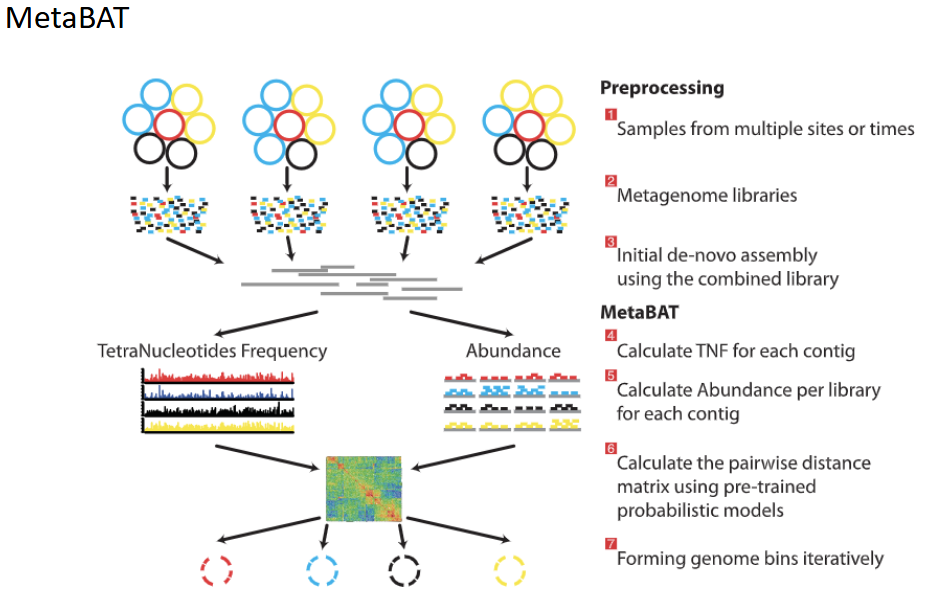
\includegraphics[width = 0.8\textwidth]{figs/metabat.png}
\end{figure}

\section{Práctica}
Esta práctica se realiza en la máquina virtual. El primer paso es crear un entorno de conda. Para ello, utilizamos el comando \texttt{conda create -n ngs python=3.11 -y}.

Podemos iniciar el entorno con \texttt{conda activate ngs} y es recomendable instalar GDown para poder descargar ficheros desde Google Drive: \texttt{pip install gdown}.

Vamos a trabajar con los datos de ECTV. Los descargamos con 

\texttt{gdown https://drive.google.com/uc?id=1gtnWLZWdZxn6j-oDvro2sDw3YHPZI2LM} 

\texttt{unzip ECTV\_reads.zip}.

\subsection{Comprobar la integridad}
Es muy recomendable comprobar la integridad de los archivos que acabamos de descargar. MD5sum y otros programas más recientes (SHA1sum) son algoritmos que «transforman» el contenido del archivo en una cadena corta de caracteres (hashes). Los hashes no cambian a menos que se modifique el contenido de los archivos (el nombre del archivo no es relevante). Por lo tanto, es muy común que las bases de datos o las instalaciones de secuenciación proporcionen hashes MD5 a los usuarios para permitir la comprobación de la integridad.
\begin{itemize}
\item \texttt{md5sum ECTV\_R1.fastq}: fa3e37e336213d01d927df2a4f0aea12
\item \texttt{md5sum ECTV\_R2.fastq}: 8a569dc04acc87067d33d3d58b26dd6d
\end{itemize}

Por último, basta con inspeccionar los hashes a ojo para comprobar si hay algún cambio. Por lo general, si los archivos se rompen por cualquier razón, el hash md5 es completamente diferente y sólo mirando a los últimos 5-6 dígitos nos va a mostrar si algo va mal.

\subsection{Contar número de reads}
Ambos archivos deberían tener el mismo número de lecturas (Illumina paried-end reads). Es una buena práctica comprobar el número de lecturas en ambos archivos. A pesar de haber comprobado los hashes MD5, a veces, los archivos subidos a la base de datos son erróneos (el remitente puede haber subido archivos truncados en lugar de los archivos originales). Además, conocer el número de lecturas sería útil para las métricas de calidad de base (lecturas ensambladas/mapeadas o lecturas de pase de calidad).

So, the easy way of counting the number of reads in a file is using wc linux command (word count): \texttt{wc -l ECTV\_R1.fastq} y \texttt{wc -l ECTV\_R2.fastq}. Se aplica la opción -l para contar el número de líneas. Sin embargo, tenemos que dividir por 4 para obtener el número de lecturas. Para evitar esto, podemos aplicar algunos piping:
\texttt{wc -l ECTV\_R1.fastq | awk '{print \$1/4}'}. En este caso, ambos ficheros tienen 50000 líneas.

\subsection{Comprobar la calidad}
Utilizamos FastQC para comprobar la calidad de las secuencias. Se instala con \texttt{conda install -c bioconda fastqc -y}.

Ahora se ejecuta el programa: \texttt{fastqc ECTV\_R1.fastq -o ECTV\_Quality/}.

Podemos utilizar las opciones -t para aumentar el número de hilos que utilizará el programa (no es necesario en este pequeño conjunto de datos).

Abra los archivos html para obtener información sobre el número de secuencias, la distribución de longitudes, el contenido de \%GCs, la calidad media, etc.

Todos los ticks están en verde salvo "Per base sequence content", pero esto no es preocupante al tratarse de un virus. Esto depende de la naturaleza de la especie de estudio. 